\documentclass[12pt, xcolor=dvipsnames]{scrartcl}
\usepackage[utf8]{inputenc}
\usepackage{mathptmx}
\usepackage[T1]{fontenc}
\usepackage{lmodern}
\usepackage{graphicx}
\usepackage[english]{babel}
\usepackage[draft=false, kerning=true]{microtype} 
\usepackage{amsmath, amssymb, amstext, amsthm}
\usepackage{hyperref}
\usepackage[a4paper,left=2.6cm, right=2.9cm,top=3.5cm, bottom=3.5cm]{geometry}
\addtokomafont{sectioning}{\rmfamily} %Titelzeilen
\theoremstyle{definition}
\newtheorem{definition}{Definition}%[section]
\newtheorem*{formulierung}{Formulierung}%[section]
\newtheorem*{theorem}{Satz}
\usepackage{physics}
\usepackage{mathtools}
\usepackage[dvipsnames]{xcolor}
\usepackage{color}
\usepackage{tikz}
%\usepackage{pgf-pie}
\usetikzlibrary{arrows.meta}
\usetikzlibrary{calc}
\usepackage{verbatim}
\usetikzlibrary{arrows,shapes}
\usepackage{graphics}
\usepackage{parskip}
\usepackage[onehalfspacing]{setspace} % 1.5 Zeilenabstand
\usepackage[justification=centering]{caption}
\usepackage{enumitem}
\usepackage[sort&compress,numbers]{natbib}
\usepackage{caption}
\usepackage{subcaption}
\usepackage{booktabs, makecell}
\usepackage{float}
\usepackage{listings}
\usepackage{colortbl} 
\usepackage{xfrac}
\usepackage{array}
\usepackage{pgfplots}
\usepackage{ulem}
\usepackage{listings}
\usepackage{romannum}
\usepackage{xcolor}
\usepackage{multicol}
\usepackage{calc}
\usetikzlibrary{positioning,matrix, arrows.meta}

\tikzset{
    table nodes/.style={
        draw,
        align=center,
        minimum height=7mm,
        minimum width =7mm,
        text depth=0.5ex,
        text height=2ex
    },      
    table/.style={
        matrix of nodes,
        row sep=-\pgflinewidth,
        column sep=-\pgflinewidth,
        nodes={
            table nodes
          },
        nodes in empty cells
     }
}


\definecolor{codegreen}{rgb}{0,0.6,0}
\definecolor{codegray}{rgb}{0.5,0.5,0.5}
\definecolor{codepurple}{rgb}{0.58,0,0.82}
\definecolor{mygreen}{RGB}{28,172,0} % color values Red, Green, Blue
\definecolor{mylilas}{RGB}{170,55,241}
\definecolor{backcolour}{rgb}{0.95,0.95,0.92}

\theoremstyle{definition}
%\newtheorem{definition}{Definition}

\title{A polynomial-Time Algorithm for the Maximum Clique Problem}
\subtitle{Detailed overview}
\author{Zohreh O. Akbari}
\date{\today}

\begin{document}
\pagenumbering{arabic}
\maketitle

\newpage

\subsection*{\Romannum{1}. Introduction}
An important consequence of the Cook-Levin theorem claims, that if any NP-complete problem can be solved in polynomial time, then every problem in NP has a polynomial-time solution. Thus besides many important applications in different domains, a polynomial-time solution to the maximum clique problem, as an NP-complete problem causes every problem in NP to have a polynomial solution, which leads to the equality of P and NP complexity classes.

This paper presents a polynomial-time algorithm for the \textit{maximum clique problem}, which detects the maximum clique of a given graph through a recursive approach.

\subsection*{\Romannum{2}. The Maximum Clique Problem}

\begin{definition}[Graph]\ \\
    Let $V$ be a set of vertices and $E \subseteq \{ \{i,j\} \mid i,j \in V, i \neq j\}$ a set of edges. The pair $G = (V,E)$ is called a graph.
\end{definition}

\begin{definition}[Complete graph]\ \\
    A graph $G = (V,E)$ is called complete graph, if every pair of distinct vertices is connected by a unique edge. That means $\forall ~ i,j \in V,~ i \neq j \Longrightarrow (i,j) \in E$. A graph is complete, if and only if every vertex has degree $|V|-1$. All complete graphs are their own maximal cliques.
    
    The author defines the complete graph by $\varphi$.
\end{definition}

\begin{definition}[Clique]\ \\
    Let $C \subseteq V$. $C$ is called a clique, if and only if  $G = (C,E')$ is complete.
\end{definition}

\begin{definition}[Maximum clique]\ \\
    The maximum clique of $G$ is called $\omega (G)$. That means  
    \[ \omega (G) = \max\{|S| : S \text{ is a clique in }G\} \]
\end{definition}

\begin{definition}[Largest subgraph of $G$ in which $\alpha$ exists]\ \\
    Let $\alpha$ be the vertex of lowest degree:
    \[ \alpha = \{j \in V : deg(j) \text{ is minimal}\} \]
    The author calls the subgraph, which contains $\alpha$ and all connected vertices to $\alpha$, the largest subgraph of $G$ in which $\alpha$ exists.

    \textit{($\alpha$ and all his neighbours including edges)}
\end{definition}

\subsection*{\Romannum{3}. A Polynomial-Time Algorithm for the Maximum Clique Problem}

Pseudocode:

\lstdefinestyle{mystyle}{
    backgroundcolor=\color{backcolour},   
    commentstyle=\color{codegreen},
    keywordstyle=\color{blue},
    numberstyle=\tiny\color{codegray},
    stringstyle=\color{codepurple},
    basicstyle=\ttfamily\footnotesize,
    breakatwhitespace=false,         
    breaklines=true,                 
    captionpos=b,                    
    keepspaces=true,                 
    numbers=left,                    
    numbersep=5pt,                  
    showspaces=false,                
    showstringspaces=false,
    showtabs=false,                  
    tabsize=2,
    aboveskip=\medskipamount,
    moredelim=**[is][\color{blue}]{@}{@},
    moredelim=**[is][\color{codepurple}]{€}{€}
}

\lstset{style=mystyle}

\begin{lstlisting}[escapeinside={(*}{*)}]
€MaxClique€(G) {
    @if@ (G is a complete graph)
        @for each@ vertex of G: v
            @if@ (|V| - 1 > max C[v])
                max C[v] := |V|;
                make max CP[v] point to a linked list containing V;
    @else@
    find the vertex of lowest degree: (*$\alpha$*)
    find the largest subgraph of G in which (*$\alpha$*) exists: G'(V',E')
    €MaxClique€(G');
    @if@ (V - (*$\alpha \neq \varphi$*))
        €MaxClique€(G - (*$\alpha$*));
}
\end{lstlisting}

\newpage

Auhtors example: 

          \begin{figure}[H]
            \centering
          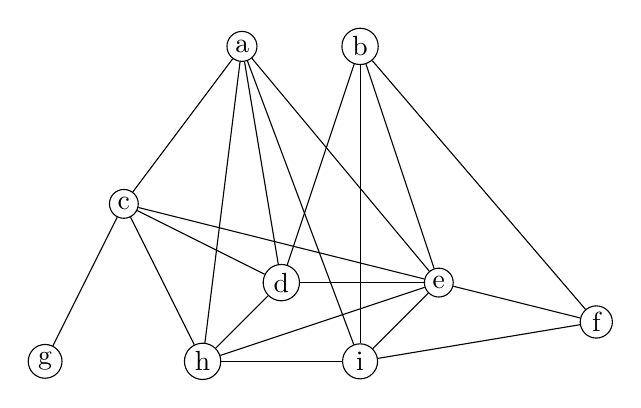
\begin{tikzpicture}
            \draw (2.5,4) node[draw, circle, inner sep=1.5pt]               (a) {a};
            \draw (4,4) node[draw, circle, inner sep=1.5pt]                   (b) {b};
            \draw (1,2) node[draw, circle, inner sep=1.5pt]                  (c) {c};
            \draw (3,1) node[draw, circle, inner sep=1.5pt]                  (d) {d};
            \draw (5,1) node[draw, circle, inner sep=1.5pt]                  (e) {e};
            \draw (7,0.5) node[draw, circle, inner sep=1.5pt]                  (f) {f};
            \draw (0,0) node[draw, circle, inner sep=1.5pt]                    (g) {g};
            \draw (2,0) node[draw, circle, inner sep=1.5pt]                  (h) {h};
            \draw (4,0) node[draw, circle, inner sep=2pt]                  (i) {i};
            \draw (g) -- (c);
            \draw (c) -- (a);
            \draw (c) -- (e);
            \draw (c) -- (d);
            \draw (c) -- (h);
            \draw (h) -- (d);
            \draw (h) -- (a);
            \draw (h) -- (i);
            \draw (i) -- (a);
            \draw (i) -- (b);
            \draw (i) -- (e);
            \draw (i) -- (f);
            \draw (f) -- (e);  
            \draw (f) -- (b);
            \draw (e) -- (b);
            \draw (e) -- (a);
            \draw (d) -- (e);
            \draw (d) -- (a);
            \draw (d) -- (b);
            \draw (h) -- (e);

            \end{tikzpicture}
            \caption{Graph $G$}
          \end{figure}

          We start with this arbitrary graph $G$. \\ 
          $G$ is not complete. Therefor we choose the vertex of minimal degree, which is $g$. That means $\alpha := g$. \\
          Now we determine the largest subgraph $G'$ of $G$, which contains $\alpha$.

        \begin{figure}[H]
          \centering
            \begin{minipage}[c]{6cm}
                $G' = (\{c,g\},\{\{c,g\}\})$ 
            \end{minipage}%
            \begin{minipage}[c]{\textwidth-7cm}
                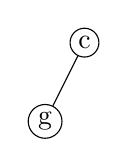
\begin{tikzpicture}
                    \draw (0.5,1) node[draw, circle, inner sep=1.5pt]                  (c) {c};
                    \draw (0,0) node[draw, circle, inner sep=1.5pt]                    (g) {g};
                    \draw (g) -- (c);
                    \end{tikzpicture}
            \end{minipage}
            \caption{Largest subgraph $G'$ which contains $g$}
         \end{figure}

         $G'$ is complete. Therefor we updated the list and linked list, which was empty. The vertices $c$ and $g$ have value 2 and point to the linked list, which contains the clique we found. 

         \begin{figure}[H]
          \centering
         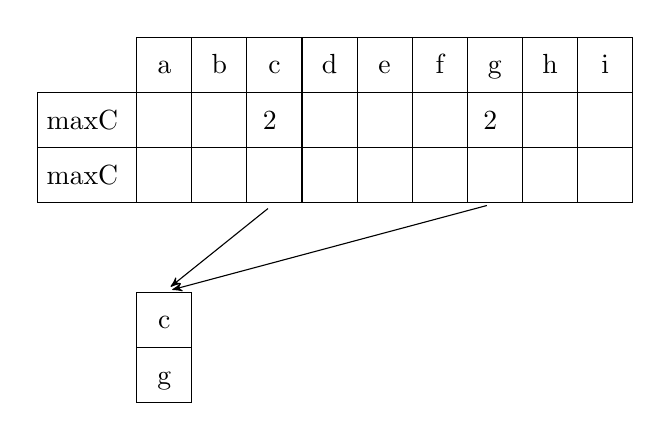
\begin{tikzpicture}
            \matrix[table] (A)
            { |[draw=none]|
                  &a&b&c&d&e&f&g&h&i\\
              maxC &  &  & 2 &  &  &  & 2 &  &  \\
              maxC & & & & & & & & & \\
            };
            \matrix[table,below=of A-3-2] (B) {c\\g\\};
            %\matrix[table,below=of A-3-6] (C) {b\\e\\f\\i\\};
            %\matrix[table,below=of A-3-8] (D) {a\\c\\d\\e\\};
            \foreach \s/\t in {8/B,4/B}%,3/C,7/C,10/C,2/D,4/D,5/D,6/D,9/D}
              \draw[-stealth',shorten >=3pt,shorten <=3pt] (A-3-\s.south) -- (\t-1-1.north);
          \end{tikzpicture}
          \caption{Updated list}
        \end{figure}

          Now we remove $\alpha$ from the graph $G$ and we can see that $G - g$ is not complete.\\

          \begin{figure}[H]
            \centering
          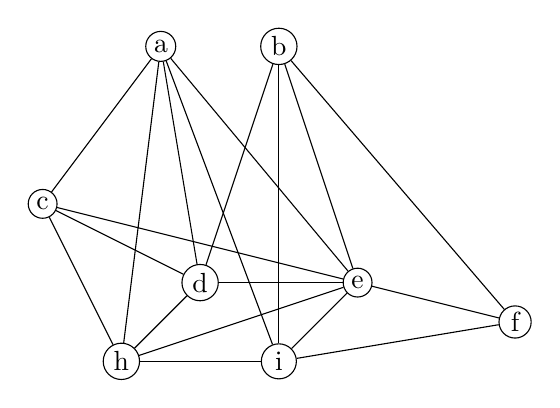
\begin{tikzpicture}
            \draw (2.5,4) node[draw, circle, inner sep=1.5pt]               (a) {a};
            \draw (4,4) node[draw, circle, inner sep=1.5pt]                   (b) {b};
            \draw (1,2) node[draw, circle, inner sep=1.5pt]                  (c) {c};
            \draw (3,1) node[draw, circle, inner sep=1.5pt]                  (d) {d};
            \draw (5,1) node[draw, circle, inner sep=1.5pt]                  (e) {e};
            \draw (7,0.5) node[draw, circle, inner sep=1.5pt]                  (f) {f};
            \draw (2,0) node[draw, circle, inner sep=1.5pt]                  (h) {h};
            \draw (4,0) node[draw, circle, inner sep=2pt]                  (i) {i};
            \draw (c) -- (a);
            \draw (c) -- (e);
            \draw (c) -- (d);
            \draw (c) -- (h);
            \draw (h) -- (d);
            \draw (h) -- (a);
            \draw (h) -- (i);
            \draw (i) -- (a);
            \draw (i) -- (b);
            \draw (i) -- (e);
            \draw (i) -- (f);
            \draw (f) -- (e);  
            \draw (f) -- (b);
            \draw (e) -- (b);
            \draw (e) -- (a);
            \draw (d) -- (e);
            \draw (d) -- (a);
            \draw (d) -- (b);
            \draw (h) -- (e);

            \end{tikzpicture}
            \caption{$G - g$}
          \end{figure}

          Therefor we obtain the vertex of minimal degree, which is $f$. That means $\alpha := f$. The largest subgraph, which contains $f$ looks like follows:\\
          
          $G' = (\{b,e,f,i\},\{\{b,e\},\{b,f\},\{b,i\},\{e,f\},\{e,i\},\{f,i\}\})$ 
          \begin{figure}[H]
            \centering
          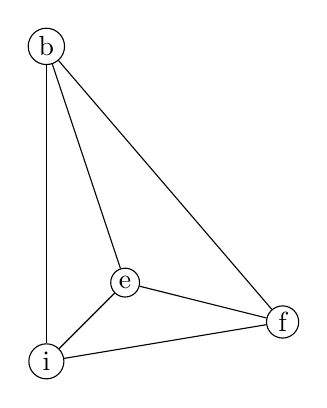
\begin{tikzpicture}
            \draw (4,4) node[draw, circle, inner sep=1.5pt]                   (b) {b};
            \draw (5,1) node[draw, circle, inner sep=1.5pt]                  (e) {e};
            \draw (7,0.5) node[draw, circle, inner sep=1.5pt]                  (f) {f};
            \draw (4,0) node[draw, circle, inner sep=2pt]                  (i) {i};
            \draw (i) -- (b);
            \draw (i) -- (e);
            \draw (i) -- (f);
            \draw (f) -- (e);  
            \draw (f) -- (b);
            \draw (e) -- (b);

            \end{tikzpicture}
            \caption{Largest subgraph $G'$ which contains $f$}
          \end{figure}

          $G'$ is complete and we can update the list.

          \begin{figure}[H]
            \centering
         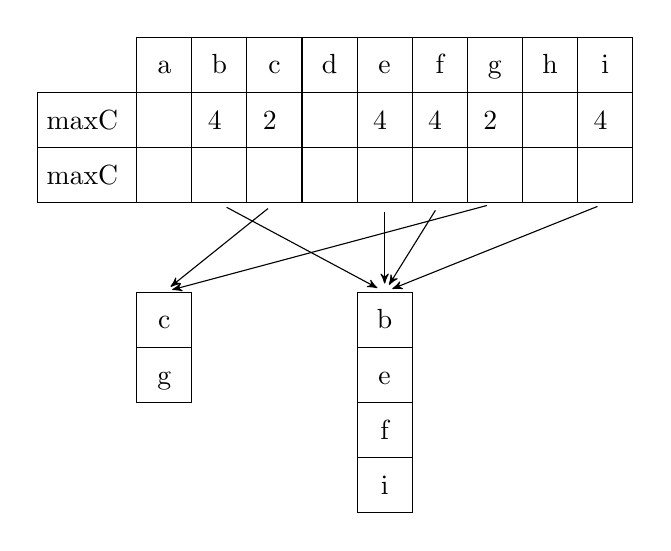
\begin{tikzpicture}
            \matrix[table] (A)
            { |[draw=none]|
                  &a&b&c&d&e&f&g&h&i\\
              maxC &  & 4 & 2 &  & 4 & 4 & 2 &  & 4 \\
              maxC & & & & & & & & & \\
            };
            \matrix[table,below=of A-3-2] (B) {c\\g\\};
            \matrix[table,below=of A-3-6] (C) {b\\e\\f\\i\\};
            %\matrix[table,below=of A-3-8] (D) {a\\c\\d\\e\\};
            \foreach \s/\t in {8/B,4/B,3/C,6/C,7/C,10/C}%,3/C,7/C,10/C,2/D,4/D,5/D,6/D,9/D}
              \draw[-stealth',shorten >=3pt,shorten <=3pt] (A-3-\s.south) -- (\t-1-1.north);
          \end{tikzpicture}
          \caption{Updated list}
        \end{figure}

          Now we remove $\alpha$ from the graph $G$ and we can see that $G - f$ is not complete.\\

          \begin{figure}[H]
            \centering
          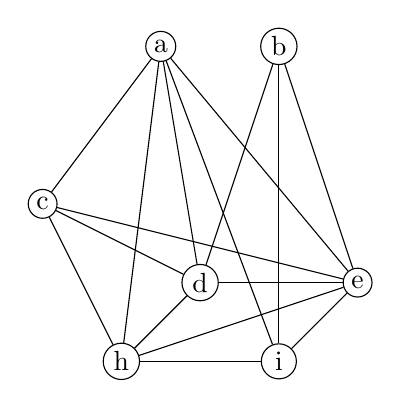
\begin{tikzpicture}
            \draw (2.5,4) node[draw, circle, inner sep=1.5pt]               (a) {a};
            \draw (4,4) node[draw, circle, inner sep=1.5pt]                   (b) {b};
            \draw (1,2) node[draw, circle, inner sep=1.5pt]                  (c) {c};
            \draw (3,1) node[draw, circle, inner sep=1.5pt]                  (d) {d};
            \draw (5,1) node[draw, circle, inner sep=1.5pt]                  (e) {e};
            \draw (2,0) node[draw, circle, inner sep=1.5pt]                  (h) {h};
            \draw (4,0) node[draw, circle, inner sep=2pt]                  (i) {i};
            \draw (c) -- (a);
            \draw (c) -- (e);
            \draw (c) -- (d);
            \draw (c) -- (h);
            \draw (h) -- (d);
            \draw (h) -- (a);
            \draw (h) -- (i);
            \draw (i) -- (a);
            \draw (i) -- (b);
            \draw (i) -- (e);
            \draw (e) -- (b);
            \draw (e) -- (a);
            \draw (d) -- (e);
            \draw (d) -- (a);
            \draw (d) -- (b);
            \draw (h) -- (e);

            \end{tikzpicture}
            \caption{$G - f$}
          \end{figure}

          Therefor we obtain the vertex of minimal degree, which is $b$. That means $\alpha := b$. The largest subgraph, which contains $b$ looks like follows:\\
          $G' = (\{b,d,e,i\},\{\{b,e\},\{b,d\},\{b,i\},\{d,e\},\{e,i\}\})$ 
          \begin{figure}[H]
            \centering
          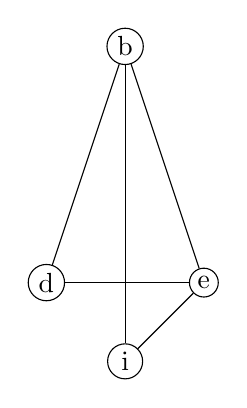
\begin{tikzpicture}
            \draw (4,4) node[draw, circle, inner sep=1.5pt]                   (b) {b};
            \draw (5,1) node[draw, circle, inner sep=1.5pt]                  (e) {e};
            \draw (3,1) node[draw, circle, inner sep=1.5pt]                  (d) {d};
            \draw (4,0) node[draw, circle, inner sep=2pt]                  (i) {i};
            \draw (i) -- (b);
            \draw (i) -- (e);
            \draw (d) -- (e);  
            \draw (d) -- (b);
            \draw (e) -- (b);

            \end{tikzpicture}
            \caption{Largest subgraph $G'$ which contains $b$}
            \label{fig:third-step}
          \end{figure}

          Now we can see that $G'$ is not complete. Therefor we repeat the algorithm on this graph \\
          There are two vertices with the same minimal degree, which is two. We can choose $d$ or $i$. For such case there is no explanation in the paper. We assume that one can choose the vertex at random. In this case we choose $\alpha := d$. Later on there will be the same example but with choice for $i$.
          \\
          $G' = (\{b,d,e\},\{\{b,e\},\{b,d\},\{d,e\}\})$ 

          \begin{figure}[H]
            \centering
          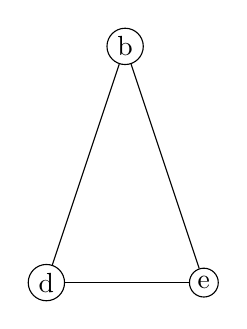
\begin{tikzpicture}
            \draw (4,4) node[draw, circle, inner sep=1.5pt]                   (b) {b};
            \draw (5,1) node[draw, circle, inner sep=1.5pt]                  (e) {e};
            \draw (3,1) node[draw, circle, inner sep=1.5pt]                  (d) {d};
            \draw (d) -- (e);  
            \draw (d) -- (b);
            \draw (e) -- (b);

            \end{tikzpicture}
            \caption{Largest subgraph $G'$ of graph in Figure \ref{fig:third-step} which contains  $d$ }
          \end{figure}


          $G'$ is complete and we can update the list. $b$ and $e$ have value four. They will not be updated, because the condition $|V| - 1 >$ max $C[v]$ is not satisfied. In this case $|V| - 1 = 2$ and $C[b] = 4$ also $C[e] = 4$. That is the reason, why only $d$ is pointing to the new clique. \\

          \begin{figure}[H]
            \centering
         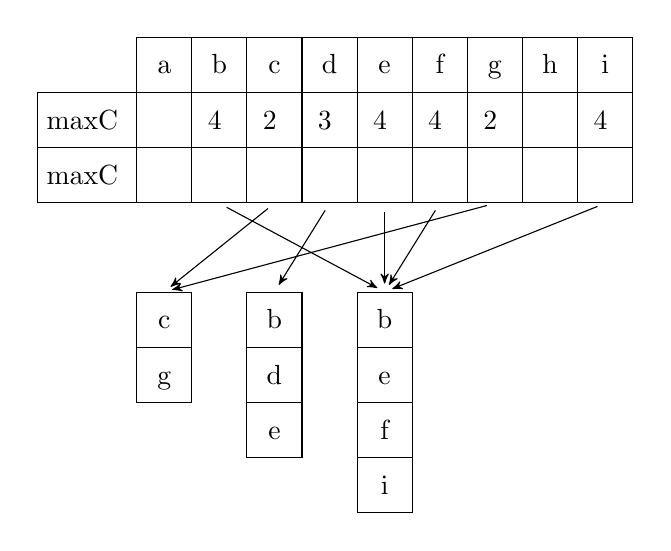
\begin{tikzpicture}
            \matrix[table] (A)
            { |[draw=none]|
                  &a&b&c&d&e&f&g&h&i\\
              maxC &  & 4 & 2 & 3 & 4 & 4 & 2 &  & 4 \\
              maxC & & & & & & & & & \\
            };
            \matrix[table,below=of A-3-2] (B) {c\\g\\};
            \matrix[table,below=of A-3-6] (C) {b\\e\\f\\i\\};
            \matrix[table,below=of A-3-4] (D) {b\\d\\e\\};
            \foreach \s/\t in {8/B,4/B,3/C,6/C,7/C,10/C,5/D}%,3/C,7/C,10/C,2/D,4/D,5/D,6/D,9/D}
              \draw[-stealth',shorten >=3pt,shorten <=3pt] (A-3-\s.south) -- (\t-1-1.north);
          \end{tikzpicture}
          \caption{Updated list}
        \end{figure}

         Now we have a look on the graph in Figure \ref{fig:third-step}. We remove the vertex $d$ and see that the new graph is complete. $(G' - d) = (\{b,e,i\},\{\{b,e\},\{b,i\},\{e,i\}\})$.  \\

          
          \begin{figure}[H]
            \centering
            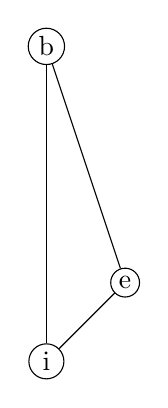
\begin{tikzpicture}
              \draw (4,4) node[draw, circle, inner sep=1.5pt]                   (b) {b};
              \draw (5,1) node[draw, circle, inner sep=1.5pt]                  (e) {e};
              \draw (4,0) node[draw, circle, inner sep=2pt]                  (i) {i};
              \draw (b) -- (e);  
              \draw (e) -- (i);
              \draw (i) -- (b);

  
              \end{tikzpicture}
              \caption{Graph in Figure \ref{fig:third-step} with removed $d$}
              \label{fig:removed-d}
            \end{figure}
            In this case the conditions for all vertices in the clique in Figure \ref{fig:removed-d} are not satisfied. Therefor there is no vertex which has to be updatetd. The list and linked list stay the same as before.

            Now we remove $\alpha$ from the graph $G$ and we can see that $G - b$ is not complete. \\

            \begin{figure}[H]
            \centering
          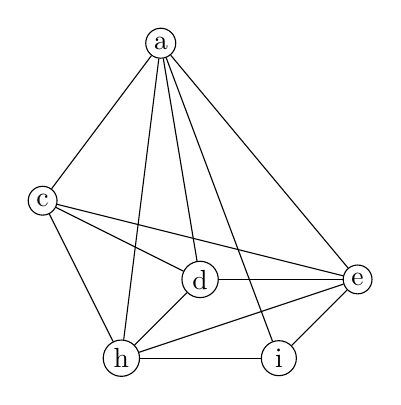
\begin{tikzpicture}
            \draw (2.5,4) node[draw, circle, inner sep=1.5pt]               (a) {a};
            \draw (1,2) node[draw, circle, inner sep=1.5pt]                  (c) {c};
            \draw (3,1) node[draw, circle, inner sep=1.5pt]                  (d) {d};
            \draw (5,1) node[draw, circle, inner sep=1.5pt]                  (e) {e};
            \draw (2,0) node[draw, circle, inner sep=1.5pt]                  (h) {h};
            \draw (4,0) node[draw, circle, inner sep=2pt]                  (i) {i};
            \draw (c) -- (a);
            \draw (c) -- (e);
            \draw (c) -- (d);
            \draw (c) -- (h);
            \draw (h) -- (d);
            \draw (h) -- (a);
            \draw (h) -- (i);
            \draw (i) -- (a);
            \draw (i) -- (e);
            \draw (e) -- (a);
            \draw (d) -- (e);
            \draw (d) -- (a);
            \draw (h) -- (e);

            \end{tikzpicture}
            \caption{$G - b$}
          \end{figure}

          We obtain the vertex of minimal degree, which is $i$. That means $\alpha := i$. The largest subgraph, which contains $i$ looks like follows:\\
          $G' = (\{a,e,i,h\},\{\{a,e\},\{a,i\},\{a,h\},\{e,i\},\{e,h\},\{i,h\}\})$ 

          \begin{figure}[H]
            \centering
          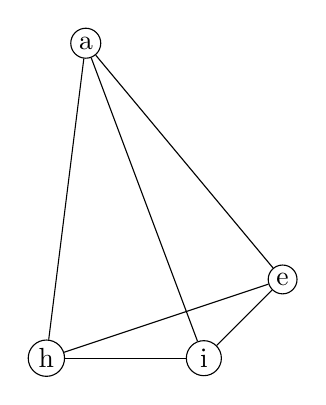
\begin{tikzpicture}
            \draw (2.5,4) node[draw, circle, inner sep=1.5pt]               (a) {a};{d};
            \draw (5,1) node[draw, circle, inner sep=1.5pt]                  (e) {e};
            \draw (2,0) node[draw, circle, inner sep=1.5pt]                  (h) {h};
            \draw (4,0) node[draw, circle, inner sep=2pt]                  (i) {i};
            \draw (e) -- (a);
            \draw (i) -- (a);
            \draw (h) -- (a);
            \draw (e) -- (i);
            \draw (i) -- (h);
            \draw (e) -- (h);
  
            \end{tikzpicture}
            \caption{Largest subgraph $G'$ which contains $i$}
            \label{fig:contains-i}
          \end{figure}

          We can see that the graph in figure \ref{fig:contains-i} is complete. Therefor it is a clique and the list will be updtated as follows: \\
         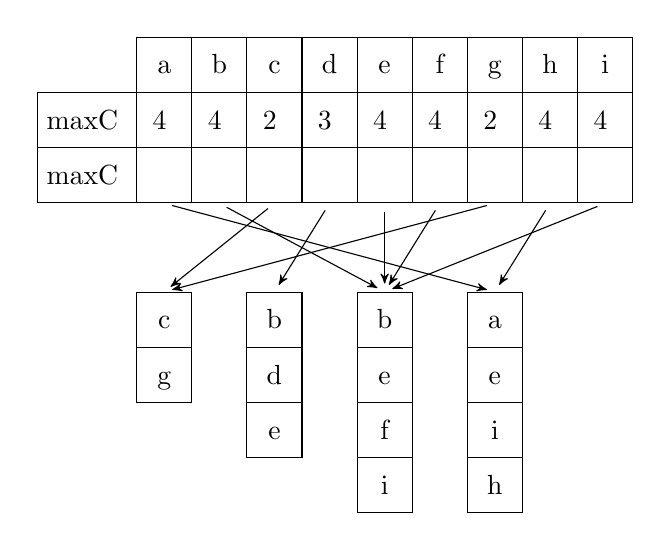
\begin{tikzpicture}
            \matrix[table] (A)
            { |[draw=none]|
                  &a&b&c&d&e&f&g&h&i\\
              maxC & 4 & 4 & 2 & 3 & 4 & 4 & 2 & 4 & 4 \\
              maxC & & & & & & & & & \\
            };
            \matrix[table,below=of A-3-2] (B) {c\\g\\};
            \matrix[table,below=of A-3-6] (C) {b\\e\\f\\i\\};
            \matrix[table,below=of A-3-4] (D) {b\\d\\e\\};
            \matrix[table,below=of A-3-8] (E) {a\\e\\i\\h\\};
            \foreach \s/\t in {8/B,4/B,3/C,6/C,7/C,10/C,5/D,2/E,9/E}
              \draw[-stealth',shorten >=3pt,shorten <=3pt] (A-3-\s.south) -- (\t-1-1.north);
          \end{tikzpicture}

          $G - i$ is a complete graph. 

          \begin{figure}[H]
            \centering
          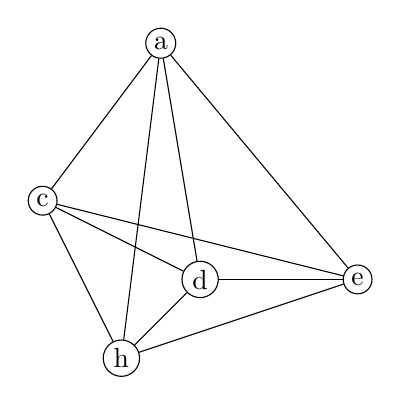
\begin{tikzpicture}
            \draw (2.5,4) node[draw, circle, inner sep=1.5pt]               (a) {a};
            \draw (1,2) node[draw, circle, inner sep=1.5pt]                  (c) {c};
            \draw (3,1) node[draw, circle, inner sep=1.5pt]                  (d) {d};
            \draw (5,1) node[draw, circle, inner sep=1.5pt]                  (e) {e};
            \draw (2,0) node[draw, circle, inner sep=1.5pt]                  (h) {h};

            \draw (c) -- (a);
            \draw (c) -- (e);
            \draw (c) -- (d);
            \draw (c) -- (h);
            \draw (h) -- (d);
            \draw (h) -- (a);
            \draw (e) -- (a);
            \draw (d) -- (e);
            \draw (d) -- (a);
            \draw (h) -- (e);

            \end{tikzpicture}
            \caption{$G - i$}
            \label{fig:finalgraph}
          \end{figure}

          The next and last step is to update the list containing the cliques.\\
          Now we have a problem at codeline 4. Let us look more closely on the if-condition:
          \[ \textbf{\texttt{if (|V| - 1 > max C[v])}} \]
          Which vertices of our clique in figure \ref{fig:finalgraph} satisfy the condition? 

          $|V| - 1 = 5 - 1 = 4$

          \begin{itemize}
            \item[\textcolor{red}{\textbullet}] $C[a] = 4 ~\ngtr~ 4$ 
            \item[\textcolor{Green}{\textbullet}] $C[c] = 4 ~>~ 2$
            \item[\textcolor{Green}{\textbullet}] $C[d] = 4 ~>~ 3$
            \item[\textcolor{red}{\textbullet}] $C[e] = 4 ~\ngtr~ 4$
            \item[\textcolor{red}{\textbullet}] $C[h] = 4 ~\ngtr~ 4$
          \end{itemize}

          The vertices $a$,$e$ and $h$ will not be updated. This is a mistake, because the vertices in the list must be part of the the maximum clique found for each vertex. In this case the maximum clique found is correct 
          but the list and linked list are not. 

          \begin{figure}[H]
            \centering
          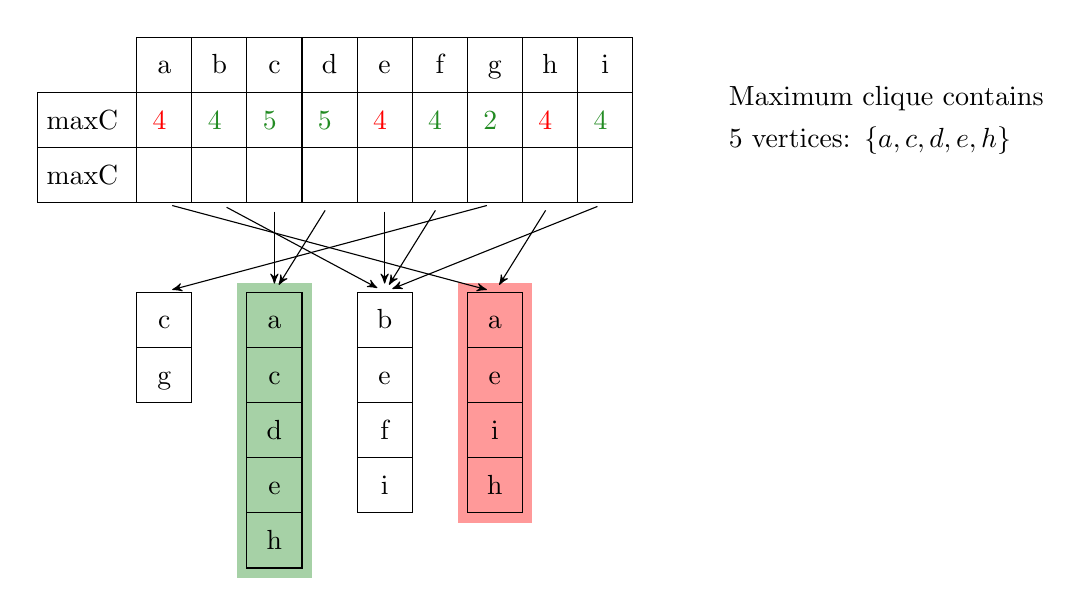
\begin{tikzpicture}
            \matrix[table] (A)
            { |[draw=none]|
                  &a&b&c&d&e&f&g&h&i\\
              maxC & \textcolor{red}{4} & \textcolor{ForestGreen}{4} & \textcolor{ForestGreen}{5} & \textcolor{ForestGreen}{5} & \textcolor{red}{4} & \textcolor{ForestGreen}{4} & \textcolor{ForestGreen}{2} & \textcolor{red}{4} & \textcolor{ForestGreen}{4} \\
              maxC & & & & & & & & & \\
            };
            \matrix[table,below=of A-3-2] (B) {c\\g\\};
            \matrix[table,below=of A-3-6] (C) {b\\e\\f\\i\\};
            \matrix[table,below=of A-3-4, fill=ForestGreen!40] (D) {a\\c\\d\\e\\h\\};
            \matrix[table,below=of A-3-8, fill=red!40 ] (E) {a\\e\\i\\h\\};
            \foreach \s/\t in {8/B,4/D,3/C,6/C,7/C,10/C,5/D,2/E,9/E}
              \draw[-stealth',shorten >=3pt,shorten <=3pt] (A-3-\s.south) -- (\t-1-1.north);
            

              \node[text width=4cm] at (7,0) 
              {Maximum clique contains $5$ vertices: $\{a,c,d,e,h\}$};
          \end{tikzpicture}
          \caption{Incorrect list and linked list}
        \end{figure}

        The red values represent the error. The green values are correct. The red colored clique should not be stated anymore. The vertices $a$ and $h$ still point to this clique because the condition is not satisfied. 


        Our assumption is that the codeline 4 must be adjusted as follows: 
        \[ \texttt{\textcolor{red}{if (|V| - 1 > max C[v])}} \text{ to } \texttt{\textcolor{Green}{if (|V| > max C[v])}} \]

        Let us repeat the last step of the example with the adjusted code. In this case we get the authors solution and the correct list:

        \[ \textbf{\texttt{if (|V| > max C[v])}} \]

        $|V| = 5 $

        \begin{itemize}
          \item[\textcolor{Green}{\textbullet}] $C[a] = 5 >~ 4$ 
          \item[\textcolor{Green}{\textbullet}] $C[c] = 5 ~>~ 2$
          \item[\textcolor{Green}{\textbullet}] $C[d] = 5 ~>~ 3$
          \item[\textcolor{Green}{\textbullet}] $C[e] = 5 ~>~ 4$
          \item[\textcolor{Green}{\textbullet}] $C[h] = 5 ~>~ 4$
        \end{itemize}

        All vertices satisfy the updated if-condition. The list looks like as follows:

        \begin{figure}[H]
          \centering
        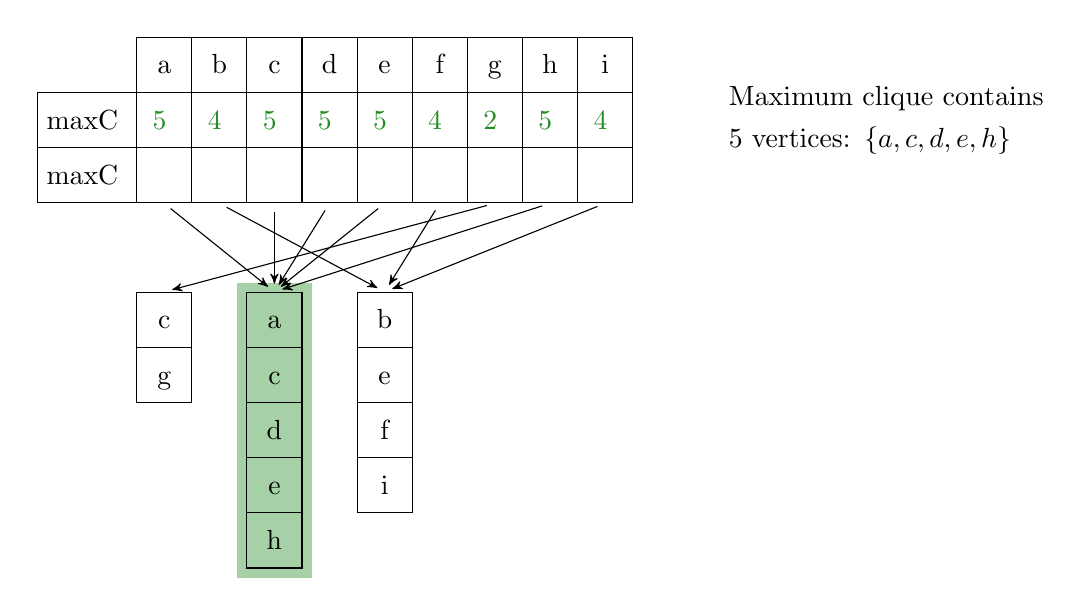
\begin{tikzpicture}
          \matrix[table] (A)
          { |[draw=none]|
                &a&b&c&d&e&f&g&h&i\\
            maxC & \textcolor{ForestGreen}{5} & \textcolor{ForestGreen}{4} & \textcolor{ForestGreen}{5} & \textcolor{ForestGreen}{5} & \textcolor{ForestGreen}{5} & \textcolor{ForestGreen}{4} & \textcolor{ForestGreen}{2} & \textcolor{ForestGreen}{5} & \textcolor{ForestGreen}{4} \\
            maxC & & & & & & & & & \\
          };
          \matrix[table,below=of A-3-2] (B) {c\\g\\};
          \matrix[table,below=of A-3-6] (C) {b\\e\\f\\i\\};
          \matrix[table,below=of A-3-4, fill=ForestGreen!40] (D) {a\\c\\d\\e\\h\\};
          \foreach \s/\t in {8/B,4/D,3/C,6/D,7/C,10/C,5/D,2/D,9/D}
            \draw[-stealth',shorten >=3pt,shorten <=3pt] (A-3-\s.south) -- (\t-1-1.north);

            \node[text width=4cm] at (7,0) 
            {Maximum clique contains $5$ vertices: $\{a,c,d,e,h\}$};
        \end{tikzpicture}
        \caption{Correct list and linked list}
        \end{figure}

        Now we get the authors solution and the algorithm stops. The maximum clique found (in both cases) is $\{a,c,d,e,h\}$.

  
   

\end{document}
